\documentclass [a4paper,10pt]{article}
\newcommand{\n}[1]{\textbf{#1}}
\newcommand{\e}[1]{\textcolor{red}{#1}}
\linespread {1.5}
\usepackage[brazilian]{babel}
\usepackage[utf8]{inputenc}
\usepackage[T1]{fontenc}
\usepackage{amsfonts}
\usepackage{amsmath}
\usepackage{amssymb}
\usepackage{caption}
\usepackage{subcaption}
\usepackage{booktabs}
\usepackage{multirow}
\usepackage{fancyhdr}
\usepackage{verbatim}
\usepackage{alltt}
\usepackage{fancyvrb}
\usepackage{graphicx,xcolor}
\usepackage{listings}
\lstset{numbers=left,
stepnumber=1,
firstnumber=1,
numberstyle=\tiny,
extendedchars=false,
breaklines=flase,
tabsize=2,
showtabs=true,
tab=\textcolor{gray}{$\cdots$},
keywordstyle=\color{blue},
frame=tb,
basicstyle=\footnotesize,
stringstyle=\ttfamily,
showstringspaces=false}
\renewcommand{\lstlistingname}{Programa}
\renewcommand{\lstlistlistingname}{Lista de Listagens}
\usepackage[pdftex]{hyperref}
\hypersetup{colorlinks,%
linkcolor=red}

\begin{document}

\noindent\rule{\textwidth}{2pt}\\[-3mm]
    \linespread {0.7} {
    \begin{Verbatim}[fontsize=\small]
    __/\\\\\\\\\\\\\\\__/\\\\\\\\\\\\\__________________/\\\_        
     _\/\\\///////////__\/\\\/////////\\\____________/\\\\\\\_       
      _\/\\\_____________\/\\\_______\/\\\___________\/////\\\_      
       _\/\\\\\\\\\\\_____\/\\\\\\\\\\\\\/________________\/\\\_     
        _\/\\\///////______\/\\\/////////__________________\/\\\_    
         _\/\\\_____________\/\\\___________________________\/\\\_   
          _\/\\\_____________\/\\\___________________________\/\\\_  
           _\/\\\\\\\\\\\\\\\_\/\\\___________________________\/\\\_ 
            _\///////////////__\///____________________________\///_     
    \end{Verbatim}
    \begin{alltt}
        \hspace{1cm} Métodos Numéricos em ALgebra Linear (MAC0300)
    \end{alltt}
    \vspace{-3mm}
    \rule{\textwidth}{2pt}\\[-6mm]

    \begin{center}
        \n{Por}\\[-0.5mm]
        $\quad${\small Caio Vinícius Dadauto$\quad$7994808}\\[-2mm]
        {\tiny \n{29/04/2014}}\\[4mm]
    \end{center}

    A implementação para a decomposição de \emph{Cholesky} foi executada em uma máquina com as seguites configurações:
    {\linespread{1}
        \begin{description}
            \item[OS] Arch Linux
            \item[Kernel] x86\_64 Linux 4.1.5-1-ARCH
            \item[CPU] Intel Core i5-4200 CPU @ 2.6GHz
            \item[RAM] 3862MiB
    \end{description}}

    {\linespread{1}
        \begin{center}
            \begin{tabular}{c c c c c c c}
                \toprule[0.11em]
                \multicolumn{7}{c}{\n{Tempo para a decomposição de \emph{Cholesky} em segundos}}\\
                \midrule
                \multirow{2}{*}{\n{Arquivos}} & \multicolumn{3}{c}{\n{Orientada a Linha}} & \multicolumn{3}{c}{\n{Orientada a Coluna}}\\
                \cmidrule(lr){2-4}
                \cmidrule(l){5-7}
                & \n{$A = GG^T$} & \n{$Gy = b$} & \n{$G^Tx = y$} & \n{$A = GG^T$} & \n{$Gy = b$} & \n{$G^Tx = y$}\\
                \cmidrule(r){1-1}
                \cmidrule(lr){2-2}
                \cmidrule(lr){3-3}
                \cmidrule(lr){4-4}
                \cmidrule(lr){5-5}
                \cmidrule(lr){6-6}
                \cmidrule(l){7-7}
                a1.dat & 0.00186 & 0.00002 & 0.00002 & 0.00200 & 0.00002 & 0.00002\\
                a2.dat & 0.01519 & 0.00008 & 0.00009 & 0.01720 & 0.00010 & 0.00009\\
                a3.dat & 0.05356 & 0.00018 & 0.00019 & 0.06334 & 0.00023 & 0.00021\\
                a4.dat & 0.13079 & 0.00035 & 0.00035 & 0.15945 & 0.00048 & 0.00038\\
                a5.dat & 0.26746 & 0.00051 & 0.00054 & 0.33196 & 0.00086 & 0.00062\\
                a6.dat & 0.47757 & 0.00074 & 0.00079 & 0.61665 & 0.00135 & 0.00092\\
                a7.dat & 0.77437 & 0.00101 & 0.00108 & 1.14896 & 0.00216 & 0.00152\\
                \toprule[0.11em]
            \end{tabular}
    \end{center}}

    A implementação para a decomposição de \emph{Cholesky} através da orientação por colunas é claramente menos eficiente
    que a implementação deste mesmo algoritimo orientado por linhas. Pois, os tempos para a orientação por
    colunas são maiores do que os tempos para a orientação por linhas. Fato  que está evidente na tabela apresentada logo
    acima. Em especial, essa diferença é mais evidente na determinação do fator de \emph{Cholesky}.

    A decomposição LU foi executada na mesma máquina em que a decomposição de \emph{Cholesky} foi executada.

    {\linespread{1}
        \begin{center}
            \begin{tabular}{c c c c c }
                \toprule[0.11em]
                \multicolumn{5}{c}{\n{Tempo para a decomposição de \emph{LU} em segundos}}\\
                \midrule
                \multirow{2}{*}{\n{Arquivos}} & \multicolumn{2}{c}{\n{Orientada a Linha}} & \multicolumn{2}{c}{\n{Orientada a Coluna}}\\
                \cmidrule(lr){2-3}
                \cmidrule(l){4-5}
                & \n{$PA = LU$} & \n{$LUx = Pb$} & \n{$PA = LU$} & \n{$LUx = Pb$}\\
                \cmidrule(r){1-1}
                \cmidrule(lr){2-2}
                \cmidrule(lr){3-3}
                \cmidrule(lr){4-4}
                \cmidrule(l){5-5}
                a1.dat & 0.00427 & 0.00009 & 0.00555 & 0.00012\\
                a2.dat & 0.01537 & 0.00017 & 0.01704 & 0.00019\\
                a3.dat & 0.05510 & 0.00037 & 0.06410 & 0.00046\\
                a4.dat & 0.12084 & 0.00065 & 0.16176 & 0.00087\\
                a5.dat & 0.23599 & 0.00106 & 0.33016 & 0.00171\\
                a6.dat & 0.40317 & 0.00149 & 0.61401 & 0.00266\\
                a7.dat & 0.64543 & 0.00208 & 1.14253 & 0.00424\\
                \toprule[0.11em]
            \end{tabular}
    \end{center}}

    As mesmas considerações feitas a respeito da diferença entre a implementação orientada por linhas e por colunas na decomposição de
    \emph{Cholesky} é feita novamente na decomposição \emph{LU}.

    \begin{figure}[!ht]
        \centering
        \begin{subfigure}[!hb]{0.5\textwidth}
            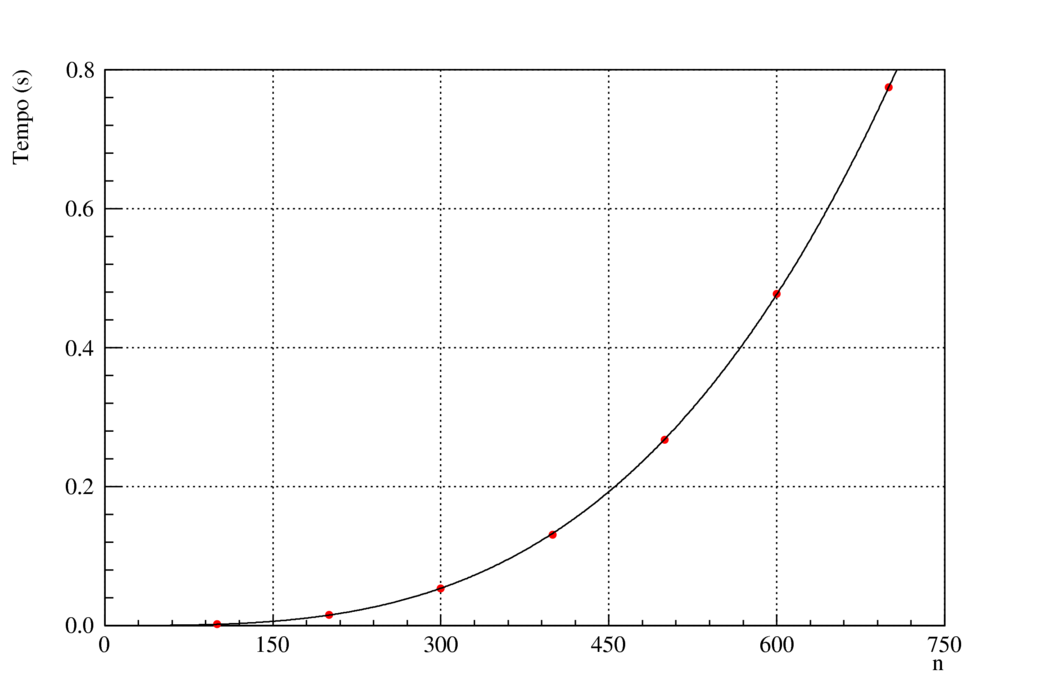
\includegraphics[width=\textwidth]{cholesky.png}
            \caption{\emph{Cholesky}.}
        \end{subfigure}%
        ~
        \begin{subfigure}[!hb]{0.5\textwidth}
            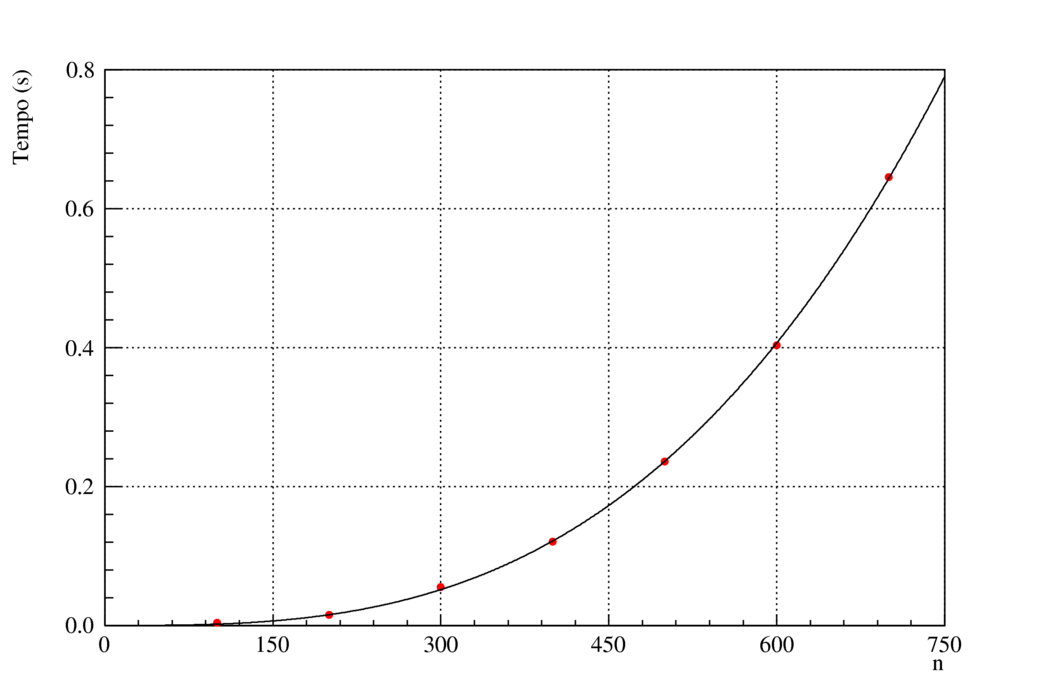
\includegraphics[width=\textwidth]{lu.png}
            \caption{\emph{LU}.}
        \end{subfigure}
        \caption{Ajuste de um polinômio da forma $[0] n^[1]$ ao tempo em função de $n$.}
    \end{figure}

    Através do ajuste por mínimos quadrados aprensentado acima, foi possível constatar que de fato a complexidade cresce com
    $O(n^3)$, uma vez que os parâmetros [1] ajustados foram, $3.15$ e $2.98$ para a decomposição de \emph{Cholesky} e \emph{LU} respectivamente.
\end{document}
    
